
\vspace{-10pt}
\section{Introduction}
\label{sec:intro}
\vspace{-10pt}

Relational databases are the most widely used database management system, underpinning much of the digital economy. Their popularity stems from their table storage structure, making maintenance relatively easy, and data simple to access using powerful query languages such as SQL. Because of their popularity, AI systems across a wide variety of domains are built using data stored in relational databases, including e-commerce, social media, banking systems, healthcare, manufacturing, and open-source scientific repositories~\citep{johnson2016mimic,pubmed}.


Despite the importance of relational databases, the rich relational information is typically foregone, as no model architecture is capable of handling varied database structures. Instead, data is ``flattened'' into a simpler format such as a single table, often by manual feature engineering, on which standard tabular models can be used~\citep{kaggle-survey}. This results in a significant loss in predictive signal, and creates a need for data extraction pipelines that frequently cause bugs and add to software complexity. 



\begin{figure*}[!t]
    \centering
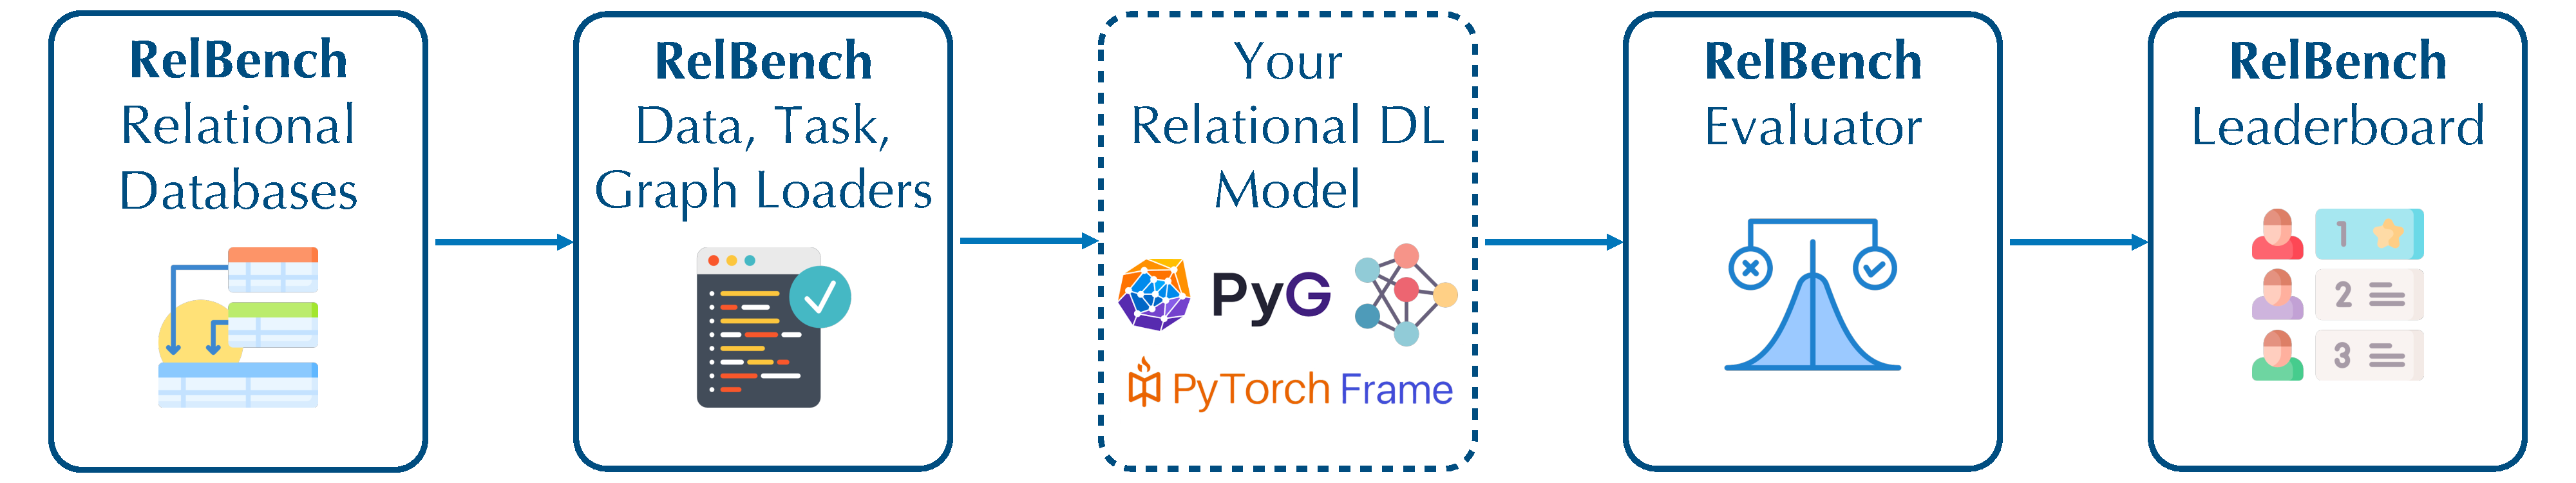
\includegraphics[width=\textwidth]{figs/relbench-fig.pdf}
    \caption{\textbf{\relbench} enables training and evaluation of deep learning models on relational databases. \relbench supports framework agnostic data loading, task specification, standardized data splitting, standardized evaluation metrics, and a leaderboard for tracking progress. \relbench also includes a pilot implementation of the relational deep learning blueprint of \cite{fey2023relational}.}
    \label{fig:rtb-fig}
    \vspace{-5pt}
\end{figure*}


%To fully exploit the predictive signal encoded in the relations between entities, a new proposal is to re-cast relational data as an exact \emph{graph} representation, with a node for each entity in the database, edges indicating primary-foreign key links, and node features extracted using deep tabular models. The graph representation allows Graph Neural Networks (GNNs)~\citep{gilmer2017mpgnn, hamilton2017inductive} to be used as predictive models, an approach termed \emph{Relational Deep Learning} (RDL)~\citep{fey2023relational}.
%\jure{This is inaccurate. RDL is not GNN on a DB graph. RDL is deep learning on a graph. I rewrote the paragraph below --- moved Fey citation a sentence earlier.}

To fully exploit the predictive signal encoded in the relations between entities, a new proposal is to re-cast relational data as an exact \emph{graph} representation, with a node for each entity in the database, edges indicating primary-foreign key links, and node features extracted using deep tabular models, an approach termed \emph{Relational Deep Learning} (RDL)~\citep{fey2023relational}. The graph representation allows Graph Neural Networks (GNNs)~\citep{gilmer2017mpgnn, hamilton2017inductive} to be used as predictive models. RDL is the first approach for an end-to-end learnable neural network model with access to all possible predictive signal in a relational databases, and has the potential to unlock new levels of predictive power.
However, the development of relational deep learning is limited by a complete lack of infrastructure to support research, including: (i) standardized benchmark databases and tasks to compare methods, (ii) initial implementation of RDL, including converting data to graph form and GNN training, and (iii) a pilot study of the effectiveness of relational deep learning. 

Here we present \relbench, the first benchmark for relational deep learning. \relbench is intended to be the foundational infrastructure for future research into relational deep learning, providing a comprehensive set of databases across a variety of domains, including \emph {e-commerce}, \emph{Q\&A platforms}, \emph{medical}, and \emph{sports} databases. \relbench databases span orders of magnitude in size, from 74K entities to 41M entities, and have very different time spans, between 2 weeks and 55 years of training data. They also vary significantly in their relational structure, with the total number of tables varying between 3 and 15, and total number of columns varying from 15 to 140.
Each database comes with multiple predictive tasks, 30 in total, including entity classification/regression and recommendation tasks, each chosen for their  real-world significance.
%\jure{can we say something about the variability: number of tables, total rows across all tables, total columns across all tables, number of predictive tasks. Let's reveal a bit more about the benchmark and get the reader excited!}
%several prediction tasks, including prediction of \emph{sales}, \emph{user value}, and \emph{user churn}, as well as \emph{recommendation} in various settings, and general \emph{entity behaviour} tasks, are defined and exposed as benchmarks. 

In addition to databases and tasks, we release open-source software designed to make relational deep learning widely available. This includes (i) the \relbench Python package for easy database and task loading, (ii) the first open-source implementation of relational deep learning, designed to be easily modified by researchers, and (iii) a public leaderboard for tracking progress. We comprehensively benchmark our initial RDL implementation on all \relbench tasks, comparing to various baselines. 

The most important baseline we compare to is a strong ``data scientist'' approach, for which we recruited an experienced individual to solve each task by manually engineering features and feeding them into tabular models. This approach is the current gold-standard for building predictive models on relational databases. The study, which we open source for reproducibility, finds that RDL models match or outperform the data scientist's models in accuracy, whilst reducing human hours worked by $96\%$, and lines of code by $94\%$ on average. This cons14titutes the first empirical demonstration of the central promise of RDL, and points to 
a long-awaited end-to-end deep learning solution for relational data.
%\jure{Can we be more specific here. Can we give the reader some answers: RDL vc DS: number of lines of code, accuracy, etc. Let's give some exciting numbers/results here.}

Our website\footnote{\website.} is a comprehensive entry point to RDL, describing \relbench databases and tasks, access to code on GitHub, the full relational deep learning blueprint, and tutorials for adding new databases and tasks to \relbench to allow researchers to experiment with their problems of interest.

